\section{Design} \label{sec:base}

A complete design---a design that detects misbehavior by both CAs and CT logs
within our strong threat model---requires a considerable degree of
complexity. In this section, we present such a full design by breaking it up
into four phases as shown in Figure~\ref{fig:design}, demonstrating the need for
the involved complexity in each step.  Later on, Section~\ref{sec:incremental}
presents two incremental versions of the full design that are less complicated
but which comes at the cost of having a weaker threat model and security goal
unless an additional CT log API is added.

A design that starts by validating SCT signatures like Apple's Safari is
promising and assumed, but it does not stand up against a malicious CA and two
CT logs that work in concert.  If the logs cannot be trusted blindly, the
presented SCTs need to be audited further.

\begin{figure*}
    \centering
	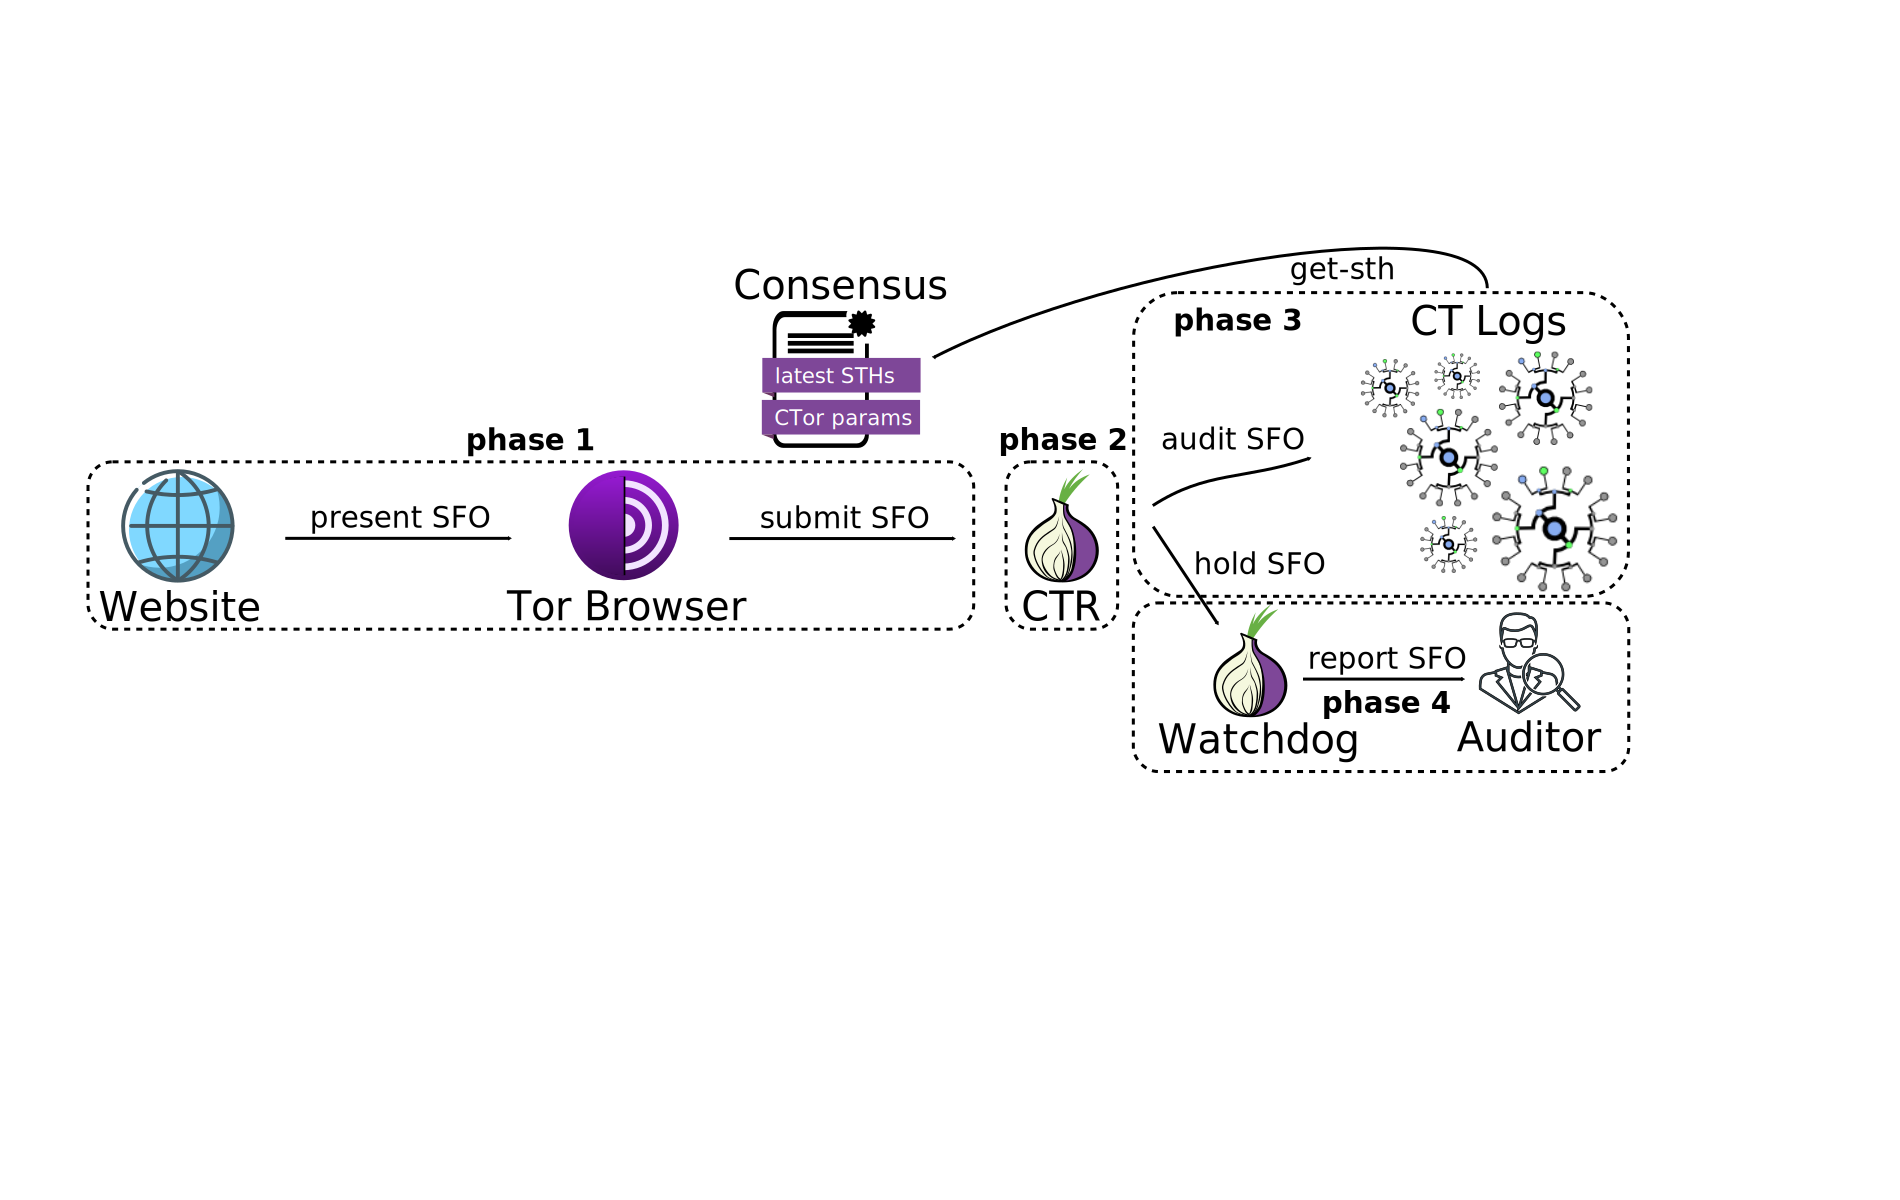
\includegraphics[width=0.8\textwidth]{img/design}
	\vspace{-8px}
	\caption{%
		An overview of the four phases of the full CTor design. In phase 1 Tor
	Browser submits a SFO (SCT Feedback Object) to a Certificate Transparency
	Relay (CTR), followed by phase 2 where the CTR buffers the SFO. In phase 3
	the relays attempts to audit the SFO, and in case of failure, it reports the
	SFO to an auditor with the help of a watchdog CTR in phase 4.}
	\label{fig:design}
	\vspace{-10px}
\end{figure*}

\subsection{Phase~1: Submission} \label{sec:base:phase1}

The least complicated auditing design would be one where Tor Browser receives a
TLS certificate and accompanying SCTs (we will refer to this bundle as an SCT
Feedback Object, or SFO for short) and talks to the corresponding logs, over
Tor, requesting an inclusion proof for each SCT. In an ordinary browser, this
would be an unacceptable privacy leak to the log of browsing behavior associated
with an IP address; performing this request over Tor hides the user's IP address
but still leaks real-time browsing behavior.

An immediate problem with this design is that a primary requirement of Tor
Browser is to persist no data about browsing behavior after the application
exits. If we assume that browsers are not left running for long periods of time,
the inclusion proof request can be easily circumvented by the attacker by using
a fresh SCT whose MMD has not completed---thus no inclusion proof needs to be
provided (yet) by the log as per the CT standard. A second problem is that the
STH that an inclusion proof refers to exists in a \emph{trust vacuum}:
	there is no way to know that it is consistent with other STHs and not part
	of a split view (assuming that there is no proactive STH
	gossip~\cite{syta,dahlberg}, which is not deployed).

We can evolve the design by adding two components: a list of STHs that Tor
Browser receives over a trusted channel and the participation of a trusted third
party with the ability to persist data and perform auditing actions at a later
point in time.

A single third party used by all users of Tor Browser would receive a
considerable aggregation of browsing behavior and would need to scale in-line
with the entire Tor network. A small number of auditors presents privacy and
single-point-of-failure concerns. A large number would be ideal but presents
difficulties in curation and independent management and still requires scaling
independent of the Tor network. These concerns do not entirely preclude the
design, but they can be easily avoided by reusing relays in the Tor Network as
our trusted third parties: we call the relays so designated Certificate
Transparency Relays (CTRs).

Now, when the browser is completing the TLS handshake, it simultaneously either
passes the SFO to a CTR (if the MMD of the SCT has not elapsed) or queries the
log itself for an inclusion proof to a trusted STH\@.  However, if we presume
the attacker can serve an exploit to the browser, the latter behavior is
immediately vulnerable. The log, upon receiving an inclusion proof request for
an SCT that it knows is malicious, can delay its response. The TLS connection in
the browser, having succeeded, will progress to the HTTP request and response,
at which point the exploit will be served, and the SFO (containing the
cryptographic evidence of CA and log misbehavior) will be deleted by the exploit
code. While blocking the TLS connection until the CT log responds is an option,
experience related to OCSP hard-fail indicates that this notion is doomed to
fail~\cite{no-hard-fail}.

The final change of the design has Tor Browser submit the SFO to the CTR
immediately upon receipt (with some probability) in all cases. A consequence of
this shift is that the trusted STH list no longer needs to be delivered to the
browser but rather the CTRs. To mitigate the risk of a browser exploit being
able to identify the CTR to the attacker (who could then target it), we prepare
\emph{CTR circuits} ahead of time that are closed and discarded as soon as the
SFO is sent. This allows the SFO submission to race with the TLS connection
completion and HTTP request/response. An added detail is to block the TLS
connection in the case that an SFO is unusually large, as defined by a parameter
\texttt{ct-large-sfo-size}. A large SFO may indicate an attempt to win the race
between SFO submission and exploitation. The parameter can be set such that it
happens extremely rarely on legitimate connections, as shown in
Section~\ref{sec:performance}.

We summarize this phase with the following algorithm that provides more explicit
steps and details, and adds a parameter \texttt{ct-submit-pr} that indicates a
probability that an SFO is submitted to a CTR. This provides probabilistic
security while providing the ability to adjust submission rates to account for
CTR and more general network scaling/health issues. Given an incoming SFO $s$,
Tor Browser should:
\begin{enumerate}
    \item Raise a certificate error and stop if the certificate chain of $s$
        is not rooted in Tor Browser's trust store.
    \item Raise a certificate transparency error and stop if the SCTs of $s$
        fail Tor Browser's CT policy.
    \item If $\mathsf{len}(s) < \texttt{ct-large-sfo-size}$, accept $s$ and
        conduct the remaining steps in the background while the TLS connection
        and subsequent HTTP request/response proceed. If $\mathsf{len}(s) \geq
        \texttt{ct-large-sfo-size}$ pause the TLS handshake, complete the
        remaining steps, accept~$s$ as valid and then continue the handshake.
    \item Flip a biased coin based on \texttt{ct-submit-pr} and stop if the
        outcome indicates no further auditing.
    \item Submit $s$ to a random CTR on a pre-built circuit. The circuit used
        for submission is closed immediately without waiting for any
        acknowledgment.
\end{enumerate}

\subsection{Phase 2: Buffering} \label{sec:base:phase2}

Once received, the most straightforward thing for a CTR to do would be to
contact the issuing log and request an inclusion proof relative to a trusted
STH\@. (And if the SCT's MMD has not elapsed, hold the SFO until it has.)
However, this proposal has two flaws, the first of which leads us to the actual
design of phase 2.

Immediately contacting the log about an SFO (i) allows the log to predict when
exactly it will receive a request about an SFO and (ii) discloses real-time
browsing behavior to the log. The former problem means that an attacker can
position resources for perpetuating an attack ahead-of-time, as well as letting
it know with certainty whether a connection was audited (based on
\texttt{ct-submit-pr}). The latter is some amount of information leakage that
can help with real-time traffic analysis.

Because a CTR must support buffering SCTs regardless (due to the MMD), we can
schedule an event in the future for when each SFO would be audited. Adding a
per-SFO value sampled from \texttt{ct-delay-dist} effectively adds stop-and-go
mixing~\cite{kesdogan:ih1998} to the privacy protection, but where there is only
one mix (CTR) between sender (client) and receiver (CT log). So there is no
point in a client-specified interval-start-time such that the mix drops messages
arriving before then, and there is no additional risk in having the interval end
time set by the mix rather than the sender. This means both that some SFOs a
client sends to a CTR at roughly the same time might be audited at different
times and that SFOs submitted to that CTR by other honest clients are more
likely to be mixed with these.

In addition to buffering SFOs for mixing effects, we also add a layer of caching
to reduce the storage overhead, prevent unnecessary log connections, and limit
the disclosure to logs. With regards to some CT circuit, an incoming SFO $s$ is
processed as follows by a CTR:
\begin{enumerate}
    \item\label{enm:storage:close} Close the circuit to enforce one-time use.
    \item\label{enm:storage:unrecognized} Discard all SCTs in the SFO for logs
        the CTR is not aware of; if no SCT remains then discard the SFO\@.
    \item\label{enm:storage:cached} Stop if $s$ is cached (see
        Section~\ref{sec:performance}) or already pending to be audited (in the
        buffer).
    \item\label{enm:storage:fix-log} Sample a CT log $l$ that issued a
        remaining SCT in~$s$.
    \item\label{enm:storage:audit-after} Compute an \texttt{audit\_after}
		time~$t$, see Figure~\ref{fig:audit-after}.
    \item\label{enm:storage:store} Add $(l,t,s)$ to a buffer of pending SFOs to
    audit.
\end{enumerate}

Recall from Section~\ref{sec:background:ct} that an inclusion proof is fetched
with regards to an STH\@.  As such, we discard SCTs that cannot be verified due
to lack of a trusted STH\@.  The sampled CT log $l$ now refers to an entity that
issued an SCT in the submitted SFO, and it will be challenged to prove inclusion
in phase~3 sometime after the \texttt{audit\_after} timestamp $t$ elapsed. We
can choose one SCT (and therefore log) at random from the SFO because it is
sufficient to suspect only one misbehaving log so long as we report the entire
SFO, allowing for other malicious logs to be identified later on (a risk
averse-attacker would not conduct an attack without controlling all necessary
logs, i.e., one benign log would else ensure public disclosure of the mis-issued
certificate).

\begin{figure}
	\centering
	\pseudocode[linenumbering, syntaxhighlight=auto]{%
		\textrm{t} \gets \mathsf{now}() +
			\mathsf{MMD} +
			\mathsf{random}(\texttt{ct-delay-dist}) \\
		\pcif \textrm{SCT.timestamp} + \textrm{MMD} <
				\mathsf{now}():\\
			\pcind\textrm{t} \gets \mathsf{now}() +
				\mathsf{random}(\texttt{ct-delay-dist})
	}
	\caption{%
		Algorithm that computes an \texttt{audit\_after} timestamp $t$.
	}
	\label{fig:audit-after}
\end{figure}

The \texttt{audit\_after} timestamp specifies the earliest point in time that an
SCT from an SFO will be audited in phase~3, which adds random noise that
obfuscates real-time browsing patterns in the Tor network and complicates
predictions of when it is safe to assume no audit will take place. If memory
becomes a scarce resource, pending triplets should be deleted at
random~\cite{nordberg}. Figure~\ref{fig:audit-after} shows that $t$ takes the
log's MMD into account. This prevents an \emph{early signal} to the issuing CT
logs that an SFO is being audited.  For example, if an SFO is audited before the
MMD elapsed, then the issuing CT log could simply merge the underlying
certificate chain to avoid any MMD violation. However, by taking the MMD into
account, this results in a relatively large time window during which the
attacker can attempt to \emph{flood} all CTRs in hope that they delete the
omitted SFO at random before it is audited. We discuss the threat of flooding
further in Section~\ref{sec:analysis:pr:phase2}, noting that such an attack can
be detected if CTRs publish two new metrics in the extra-info document:
\texttt{ct-receive-bytes} and \texttt{ct-delete-bytes}. These metrics indicate
how many SFO bytes were received and deleted throughout different time
intervals, which is similar to other extra-info metrics such as
\texttt{read-history}.

\subsection{Phase 3: Auditing} \label{sec:base:phase3}

As alluded to in phase 2, there is a second problem why the simple behavior of
``contact the log and request an inclusion proof'' is unacceptable. We include
the ability to DoS an individual Tor relay in our threat model---if the log
knows which CTR holds the evidence of its misbehavior, it can take the CTR
offline, wiping the evidence of the log's misbehavior from its memory. 

We can address this concern in a few ways. The simple proposal of contacting the
log over a Tor circuit will not suffice---a log can tag each CTR by submitting
unique SFOs to them all, and recognize the CTR when they are submitted (see
Section~\ref{sec:analysis:pr:phase3}). Even using a unique Tor circuit for each
SFO might not suffice to prevent effective tagging attacks. For example, after
tagging all CTRs, a malicious log could ignore all but innocuous untagged
requests and tagged requests matching tags for whichever CTR it decides to
respond to first. If exponential backoff\footnote{A common approach for delaying
retransmissions, often for the sake of avoiding congestion or unnecessary load.}
is supported, the rest of the CTRs will backoff repeated attempts to fetch a
proof while the probability that the first CTR is the one fetching proofs
significantly increases. The log can repeat this process---alternating tagged
CTRs it replies to---until it receives the offending SFO from a CTR with higher
probability than others. This might result in many CTRs reporting the log as
inaccessible for days, but that is not the same as direct cryptographic evidence
of misbehavior.

While there are ways to detect this attack after-the-fact, and there may be ways
to mitigate it, a more robust design would tolerate the disclosure of a CTRs
identity to the log during the auditing phase without significant security
implications.  A simple appealing approach is to write the data to disk prior
to contacting the log; however, Tor relays are explicitly designed not to write
data about user behavior to disk unless debug-level logging is enabled. Relay
operators have expressed an explicit desire to never have any user data
persisted to disk, as it changes the risk profile of their servers with regards
to search, seizure, and forensic analysis.

The final design is to have the CTR work with a partner CTR---we call it a
\emph{watchdog}---that they choose at random and contact over a circuit. Prior
to attempting to fetch a proof from a log, the CTR provides the watchdog with
the SFO it is about to audit. After an appropriate response from the log, the
CTR tells the watchdog that SFO has been adequately addressed.

In more detail, each CTR maintains a single shared circuit that is used to
interact with all CT logs known to the CTR\@. (We are not using one circuit per
SFO given the overhead and the unclear security benefit noted above.) For
\emph{each} such CT log $l$, the CTR runs the following steps indefinitely:
\begin{enumerate}
    \item\label{enm:auditing:backoff} Sample a delay $d \gets
        \mathsf{random}(\texttt{ct-backoff-dist})$ and wait until $d$ time units
        elapsed.
    \item Connect to a random watchdog CTR\@.
    \item\label{enm:auditing:loop} For each pending buffer entry $(l',s,t)$,
    where $l' = l$ and $t <= \mathsf{now}()$:
		\begin{enumerate}
			\item\label{enm:ext:auditing:watchdog} Share $s$ with the current
				watchdog.
			\item\label{enm:ext:auditing:challenge} Challenge the log to prove
                                  inclusion to the closest STH in the Tor
                                  consensus where $t$ $\leq$
                                  STH\texttt{.timestamp}. Wait at most
                                  \texttt{ct-log-timeout} time units for the
                                  complete proof to be delivered before timing
                                  out.
				\begin{itemize}
					\item\label{enm:ext:auditing:challenge:success} On valid
						proof: send an acknowledgment to the watchdog, cache $s$
						and then discard it.
					\item\label{enm:ext:auditing:challenge:fail} On any other
						outcome: close circuit to the watchdog CTR, discard $s$,
						and go to step~1.
				\end{itemize}
		\end{enumerate}
\end{enumerate}

\subsection{Phase 4: Reporting}

At any given time, a CTR may be requesting inclusion proofs from logs and act as
a watchdog for one or more other CTRs. A CTR acting as a watchdog will have at
most one SFO held temporarily for each other CTR it is interacting with. If an
acknowledgement from the other CTR is not received within
\texttt{ct-watchdog-timeout}, it becomes the watchdog's responsibility to report
the SFO for human review. In such a case, the watchdog immediately closes the
circuit to the CTR. This end-stage process that begins with the watchdog's
receipt of a suspicious SFO and culminates in human review is referred to as
auditing, and left mostly-unspecified.

Because human review and publication\footnote{Most likely on the ct-policy group
at \url{https://groups.google.com/a/chromium.org/forum/\#!forum/ct-policy}} is
critical, we envision that the watchdog (which is a Tor relay that may not be
closely monitored) provides the SFO to an independent auditor run by a human
closely monitoring its operation. When arriving at the design of the CTR being a
role played by a Tor relay, we eschewed separate auditors because of the lack of
automatic scaling with the Tor network, the considerable aggregation of browsing
behavior across the Tor network, and the difficulties of curation and validation
of trustworthy individuals. SFOs submitted to auditors at this stage have been
filtered through the CTR layer, resulting in an exponentially smaller load (and
data exposure) for auditors. This should allow for a smaller number of them to
operate without needing to scale with the network.

While we consider all auditors trusted---the watchdog needs to take precautions
talking to them because the network is not trusted (see
Section~\ref{sec:adversary}).  The watchdog can contact an auditor as soon as it
receives an SFO it should report; however it must contact the auditor over a Tor
circuit. If a successful acknowledgement from the auditor is not received within
\texttt{ct-auditor-timeout}, the SFO is buffered and should be reported again to
the same auditor over a new circuit, potentially with some modest backoff delay.

When an auditor receives an SFO, it should persist it to durable storage until
it can be successfully resolved to a specific STH\@. Once so persisted, the
auditor can begin querying the log itself asking for an inclusion proof with
regards to the \emph{first applicable STH} in the history the Tor consensus.
This prevents an attacker from hiding a MMD violation by delaying the
certificate inclusion (until the attacker knows if the SFO was selected for
auditing or not).  If no inclusion proof can be provided after some threshold of
time, or the inclusion proof shows evidence of a MMD violation, the auditor
software should raise the details to a human operator for investigation.

Separately, the auditor should be retrieving the current Tor consensus and
ensuring that a consistency proof can be provided between STHs from the older
consensus and the newer. If consistency cannot be established after some
threshold of time, the auditor software should raise the details to a human
operator for investigation. An auditor could also monitor a log's uptime and
report on excessive downtime. Finally, it is paramount that the auditor
continuously monitors its own availability from fresh Tor-circuits by submitting
known SFOs to itself to ensure that an attacker is not keeping watchdogs from
connecting to it.

\subsection{Setup} \label{sec:base:consensus}

There are a number of additional details missing to setup phases 1--4 for the
design. Most of these details relate to the Tor consensus. Directory authorities
influence the way in which Tor Browser and CTRs behave by voting on necessary
parameters, such as the probability of submission of a SFO
(\texttt{ct-submit-pr}) and the timeout used by CTRs when auditing CT logs
(\texttt{ct-log-timeout}), as introduced earlier as part of the design. See
Appendix~\ref{app:consensus-params} for details on these parameters and their
values that were previously used. Next, we briefly introduce a number of
implicitly used parts from our design that should also be part of the consensus.

In the consensus, the existing \texttt{known-flags} item determines the
different flags that the consensus might contain for relays.  We add another
flag named \texttt{CTR}, which indicates that a Tor relay should support
CT-auditing as described here. A relay qualifies as a CTR if it is flagged as
\texttt{stable} and not \texttt{exit}, to spare the relatively sparse exit
bandwidth and only use relays that can be expected to stay online.
Section~\ref{sec:privacy} discusses trade-offs in the assignment of the
\texttt{CTR} flag.

The consensus should also capture a fixed view of the CT landscape by publishing
STHs from all recognized logs.  A CT log is recognized if a majority of
directory authorities proposed a \texttt{ct-log-info} item, which contains a
log's ID, public key, base URL, MMD, and most recent STH\@.  Each directory
authority proposes its own STH, and agrees to use the most recent STH as
determined by timestamp and lexicographical order.  Since CTRs verify inclusion
with regards to SCTs that Tor Browser accepts, the CT logs recognized by Tor
Browser must be in Tor's consensus.

Tor's directory authorities also majority-vote on \texttt{ct-auditor} items,
which pin base URLs and public keys of CT auditors that watchdogs contact in
case that any log misbehavior is suspected. 
